\section{The method} \label{sec:method}

%%%%%%%%%%%%%%%%%%%%%%%%%%%%%%%%%%%%%%%%%%%%%%%%%%%%%%%%%%%%%%%%%%%%%%%%%%%%%%%%%%%%%%%%
\subsection{The $Q$ transform} \label{sec:method:qtransform}
To conduct the multi-resolution analysis motivated in the introduction, the data are processed using the $Q$ transform~\cite{Brown:1991}. The $Q$ transform is a modification of the standard short time Fourier transform in which the analysis window duration varies inversely with frequency such that the time-frequency plane is covered by tiles of constant quality factor $Q$. The signal time series, $x(t)$, is projected onto a basis of complex-valued windowed sine waves:
\begin{equation}
  X(\tau, \phi, Q) = \int_{-\infty}^{+\infty}{ x(t) w(t-\tau,\phi,Q) e^{-2i\pi\phi t}dt}.
  \label{eq:qtransform1}
\end{equation}
The transform coefficient, $X$, measures the average signal amplitude and phase within a time-frequency region, called a \textit{tile}, centered on time $\tau$ and frequency $\phi$, whose shape and area are determined by the requested quality factor $Q$ and the particular choice of analysis window, $w$. In~\cite{Gabor:1946}, it is shown that the minimal time-frequency resolution is achieved by a Gaussian window:
\begin{equation}
  w(t-\tau,\phi,Q) = \frac{W_g}{\sigma_t\sqrt{2\pi}}\exp\left [ -\frac{1}{2\sigma_t^2}(t-\tau)^2 \right],
  \label{eq:gausswindowt}
\end{equation}
where $W_g$ is a normalization factor and the Gaussian variance is $\sigma_t^2=\frac{Q^2}{8\pi^2\phi^2}$.

To optimize the algorithmic implementation of the $Q$ transform, we prefer an alternative form of Eq.~\ref{eq:qtransform1}, where we switch to the frequency domain using the Fourier transform defined as
\begin{equation}
  \tilde{x}(f) = \int_{-\infty}^{+\infty}{ x(t) e^{-2i\pi f t}dt}. \label{eq:FTforward}
\end{equation}
The corresponding reverse Fourier transform is
\begin{equation}
  x(t) = \int_{-\infty}^{+\infty}{ \tilde{x}(f) e^{2i\pi f t}df}.  \label{eq:FTbackward}
\end{equation}
Using the inverse Fourier transform, the cross-correlation theorem, the Fourier transform translation relation and the fact that we are working with a real window, we can re-write Eq~\ref{eq:qtransform1}:
\begin{align}
  X(\tau, \phi, Q) &= \int_{-\infty}^{+\infty}{\tilde{X}(f,\phi,Q) e^{+2i\pi f \tau}df} \\
  X(\tau, \phi, Q) &= \int_{-\infty}^{+\infty}{ \widetilde{\left (\int_{-\infty}^{+\infty}{w^*(t,\phi,Q)x(t+\tau)e^{-2i\pi\phi(t+\tau)}dt}\right)} e^{+2i\pi f \tau}df}\\
  X(\tau, \phi, Q) &= \int_{-\infty}^{+\infty}{ \tilde{x}(f+\phi) \tilde{w}^{*}(f,\phi,Q) e^{+2i\pi f \tau}df}.
  \label{eq:qtransform2}
\end{align}
In Eq.~\ref{eq:qtransform2}, the signal is applied a Fourier transform, a shift in frequency, a multiplication by the frequency-domain window and an inverse Fourier transform.


%%%%%%%%%%%%%%%%%%%%%%%%%%%%%%%%%%%%%%%%%%%%%%%%%%%%%%%%%%%%%%%%%%%%%%%%%%%%%%%%%%%%%%%%
\subsection{The window} \label{sec:method:window}
To compute the $Q$ transform of Eq.~\ref{eq:qtransform2}, we need to apply a Fourier transform to the Gaussian window of Eq.~\ref{eq:gausswindowt}. In the frequency domain, the window is also Gaussian and real:
\begin{equation}
  \tilde{w}(f,\phi,Q) = \tilde{w}^*(f,\phi,Q) = W_g\exp\left [ -\frac{1}{2\sigma_f^2}f^2 \right],
  \label{eq:gausswindowf}
\end{equation}
where $\sigma_f^2=\frac{2\phi^2}{Q^2}$.

The Gaussian window provides the best time-frequency resolution~\cite{Gabor:1946}. However, such a window has an infinite extent which makes it difficult to use in a discrete analysis framework. Instead, the Omicron algorithm approximates the Gaussian window with a bisquare window which has a simple form in the frequency domain:
\begin{equation}
  \tilde{w}(f,\phi,Q) = \tilde{w}^*(f,\phi,Q) =
  \begin{cases}
    W_b\left[1 - \left(\frac{f}{\delta_f(\phi,Q)}\right)^2 \right]^2 & |f| < \delta_f(\phi,Q), \\
    0 & \textrm{otherwise},
  \end{cases}
  \label{eq:bisquare}
\end{equation}
where $W_b$ is a normalization factor and $\delta_f(\phi,Q)=\phi\sqrt{11}/Q$ is the half size of the window. This window is a very good approximation to the Gaussian case~\cite{Chatterji:2004}. It achieves a time-frequency resolution that is only 4.5~\% greater than the minimum possible time-frequency uncertainty associated with the ideal Gaussian window. In addition, it offers a limited energy leakage into time-domain side lobes.

Thanks to the finite extent of the the bisquare window, it is possible to add protections against signal aliasing. Indeed, when using the two conditions
\begin{align}
  &Q\ge\sqrt{11} \qquad \text{and}\label{eq:antialias1} \\
  &\phi \le \frac{f_{\text{Nyquist}}}{1+\sqrt{11}/Q}, \label{eq:antialias2}
\end{align}
the zero frequency and the Nyquist frequency, $f_{\text{Nyquist}}$, are never exceeded: $0 \le f + \phi \le f_{\text{Nyquist}}$. The $Q$ transform in Eq.~\ref{eq:qtransform2} can, therefore, be safely discretized.

The window normalization factor is such that
\begin{equation}
  \int_{-\infty}^{+\infty}{|\tilde{w}(f,\phi,Q)|^2df} = 2.
  \label{eq:winnorm}
\end{equation}
Using this normalization condition has many advantages which will be presented in Sec.~\ref{sec:method:snr}. A trivial integration yields the normalization factor for the bisquare window
\begin{equation}
  W_b = \sqrt{\frac{315}{128\sqrt{11}} \frac{Q}{\phi}},
  \label{eq:Wb}
\end{equation}
while for the Gaussian case we get
\begin{equation}
  W_g = \sqrt{\frac{2}{\sqrt{\pi}\sigma_f}} = \sqrt{\frac{2}{\sqrt{2\pi}} \frac{Q}{\phi}},
  \label{eq:Wg}
\end{equation}

A characteristic duration, $\Delta t$, and bandwidth, $\Delta f$, are defined using the second central moments of the window:
\begin{align}
  \left(\frac{\Delta f}{2}\right)^2 &= \int_{-\infty}^{+\infty}{f^2|\tilde{w}(f,\phi,Q)|^2 df}\\
  \left(\frac{\Delta t}{2}\right)^2 &= \int_{-\infty}^{+\infty}{t^2|w(t,\phi,Q)|^2 dt}.
\end{align}
For both the Gaussian and bisquare windows, we naturally find indentical values:
\begin{align}
  \Delta f &=  2\sigma_f = 2\sqrt{2}\frac{\phi}{Q}, \\ 
  \Delta t &=  2\sigma_t = \frac{1}{\sqrt{2}\pi}\frac{Q}{\phi}.
\end{align}
Fig.~\ref{fig:window} shows a comparison between an ideal Gaussian window and its approximate using a bisquare window.
\begin{figure}
  \center
  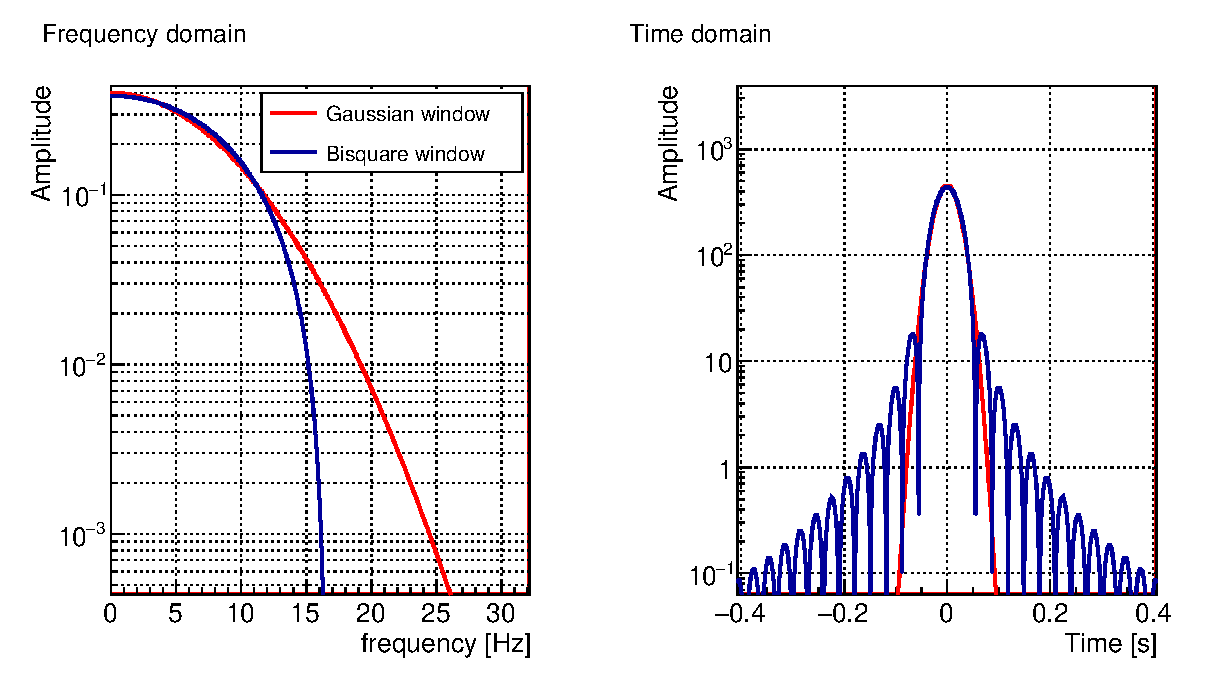
\epsfig{width=12cm, file=./figures/window.eps}
  \caption{A Gaussian window (red) is approximated by a bisquare window (blue) in the frequency domain (left) and, after an inverse Fourier transform, in the time domain (right). We used $\phi=100$~Hz and $Q=20$.}
  \label{fig:window}
\end{figure}

In the following, we will often refer to a basis of complex-valued sinusoidal Gaussian waveforms keeping in mind that bisquare windows are actually used for the Omicron implementation.


%%%%%%%%%%%%%%%%%%%%%%%%%%%%%%%%%%%%%%%%%%%%%%%%%%%%%%%%%%%%%%%%%%%%%%%%%%%%%%%%%%%%%%%%
\subsection{The tiles} \label{sec:method:tiles}
The tiles must be chosen to cover a finite region of parameter space, $[\tau_{min};\tau_{max}]\times [\phi_{min};\phi_{max}] \times [Q_{min};Q_{max}]$. The density of tiles must be large to guarantee a high detection efficiency. However, the number of tiles must also be as small as possible to provide a fast processing. To meet these two competitive requirements, the parameter space is tiled such that the fractional energy loss due to mismatch is below a pre-defined value, $\mu_{max}$. For complex-valued sinusoidal Gaussian waveforms, the mismatch can be analytically computed and the optimal number of tiles can be determined. The Omicron algorithm adopts the tiling strategy developed in~\cite{Chatterji:2004}, where the tiles are distributed over a cubic lattice using a mismatch metric\footnote{The metric includes a non-diagonal $\delta \phi \delta Q$ term which has been neglected.} to measure distances:
\begin{equation}
  \delta s^2 =
  \frac{4\pi^2\phi^2}{Q^2}\delta \tau^2
  + \frac{2+Q^2}{4\phi^2}\delta \phi^2
  + \frac{1}{2Q^2}\delta Q^2.
  \label{eq:tilemetric}
\end{equation}
To guarantee a fractional energy loss smaller than $\mu_{max}$, the minimum number of tiles, $N_\tau \times N_\phi \times N_Q$, is given by the mismatch distances integrated over the three dimensions:
\begin{align}
  N_\tau \ge \frac{s_\tau}{2\sqrt{\mu_{max}/3}},  & \qquad s_\tau = \frac{2\pi\phi}{Q}(\tau_{max} - \tau_{min}), \label{eq:tiledistancetau} \\
  N_\phi \ge \frac{s_\phi}{2\sqrt{\mu_{max}/3}},  & \qquad s_\phi = \frac{\sqrt{2+Q^2}}{2}\ln(\phi_{max}/\phi_{min}), \label{eq:tiledistancephi} \\
  N_Q \ge \frac{s_Q}{2\sqrt{\mu_{max}/3}},  & \qquad s_Q = \frac{1}{\sqrt{2}}\ln(Q_{max}/Q_{min}). \label{eq:tiledistanceq}
\end{align}
This Omicron tiling structure can be depicted as a set of $N_Q$ logarithmically-spaced $Q$ planes, indexed by $q$:
\begin{equation}
  Q_q = Q_{min}\left[ \frac{Q_{max}}{Q_{min}}\right]^{(0.5+q)/N_q}, \qquad 0\le q < N_Q.
  \label{eq:q}
\end{equation}
Each of these planes is divided into $N_\phi$ logarithmically-spaced frequency rows, indexed by $l$:
\begin{equation}
  \phi_l = \phi_{min}\left[ \frac{\phi_{max}}{\phi_{min}}\right]^{(0.5+l)/N_\phi}, \qquad 0\le l < N_\phi.
  \label{eq:phi}
\end{equation}
Each frequency row is finally sub-divided into $N_\tau$ linearly-spaced time bins, indexed by $m$:
\begin{equation}
  \tau_m = -\frac{T_c}{2}+(m+0.5)\frac{T_c}{N_\tau}, \qquad 0\le m < N_\tau.
  \label{eq:tau}
\end{equation}


%%%%%%%%%%%%%%%%%%%%%%%%%%%%%%%%%%%%%%%%%%%%%%%%%%%%%%%%%%%%%%%%%%%%%%%%%%%%%%%%%%%%%%%%
\subsection{The data whiteing} \label{sec:method:whitening}

As we will see in Sec.~\ref{sec:method:snr}, whitening the data before applying the $Q$ transform is useful for a subsequent statistical interpretation of the $Q$ transform coefficients. To achieve this, a simple method consists of re-weighting the frequency-domain data by the inverse amplitude spectral density:
\begin{equation}
  \tilde{x}_{white}(f) = \frac{\tilde{x}(f)}{\sqrt{S(|f|)}},
  \label{eq:whitening}
\end{equation}
where $S(f)$ is the one-sided ($f \ge 0$) power spectrum density (PSD). After this transformation, the power is equally distributed over the frequencies and the one-sided PSD of $x_{white}$ is flat and equal to 1. The one-sided PSD is usually estimated by averaging multiple one-sided periodograms computed over a finite duration $T$:
\begin{equation}
  P_T(f) = \frac{2}{T}\left|\tilde{x}_T(f)\right|^2, \qquad f \ge 0.
  \label{eq:periodogram}
\end{equation}
The factor 2 accounts for negative frequencies of $\tilde{x}_T$ which are ignored in a one-sided convention.


%%%%%%%%%%%%%%%%%%%%%%%%%%%%%%%%%%%%%%%%%%%%%%%%%%%%%%%%%%%%%%%%%%%%%%%%%%%%%%%%%%%%%%%%
\subsection{The signal to noise ratio} \label{sec:method:snr}

Let's consider a signal which is a burst of energy of amplitude $B$ with a sinusoidal Gaussian waveform, the parameters of which exactly match the tile indexed by $b$:
\begin{align}
  b(t) &= Bw(t-\tau_b, \phi_b, Q_b)\cos(2\pi\phi_b t + \theta_b),\\
  \tilde{b}(f) &= B\left[ \tilde{w}(f-\phi_b,\phi_b,Q_b)e^{i\theta_b}+\tilde{w}(f+\phi_b,\phi_b,Q_b)e^{-i\theta_b}\right]/2,
\end{align}
where $\theta_b$ is the arbitrary phase between the burst and tile $b$. The burst signal lives on top of a stationary stochastic noise $n(t)$: $x(t) = b(t) + n(t)$. The squared magnitude of the Q transform coefficient for tile $b$ is
\begin{equation}
  |X(\tau_b, \phi_b, Q_b)|^2 = |X_n(\tau_b, \phi_b, Q_b)|^2 + |X_b(\tau_b, \phi_b, Q_b)|^2 + 2|X_n(\tau_b, \phi_b, Q_b)|\ |X_b(\tau_b, \phi_b, Q_b)|\cos{\theta},
\end{equation}
where $X_b$ and $X_n$ are the $Q$-transform coefficients for the burst and noise components. The phase between the two signals, $\theta$, is a random variable. The last term vanishes when we consider the expectation value for multiple measurements:
\begin{equation}
  \langle |X(\tau_b, \phi_b, Q_b)|^2 \rangle= \langle |X_n(\tau_b, \phi_b, Q_b)|^2 \rangle + \langle |X_b(\tau_b, \phi_b, Q_b)|^2 \rangle.
\end{equation}
Using the frequency-domain $Q$ transform of Eq.~\ref{eq:qtransform2}, we write the burst contribution as
\begin{align}
  |X_b(\tau_b, \phi_b, Q_b)|^2 &= \left|\int_{-\infty}^{+\infty}{ \frac{B}{2}\left[ \tilde{w}(f,\phi_b,Q_b)e^{i\theta_b}+\tilde{w}(f+2\phi_b,\phi_b,Q_b)e^{-i\theta_b}\right] \tilde{w}^{*}(f,\phi_b,Q_b) e^{+2i\pi f \tau_b}df} \right|^2\\
  &= \left|\int_{-\infty}^{+\infty}{ \frac{B}{2} \tilde{w}(f,\phi_b,Q_b)e^{i\theta_b} \tilde{w}^{*}(f,\phi_b,Q_b) e^{+2i\pi f \tau_b}df}\right|^2 \\
  &= B^2
  \label{eq:qtransform_signal}
\end{align}
where we used the window normalization of~Eq.\ref{eq:winnorm} and the fact that $\tilde{w}^{*}(f,\phi_b,Q_b)\tilde{w}(f+2\phi_b,\phi_b,Q_b)=0$ if we use the bisquare window approximation and verify condition~\ref{eq:antialias1}.

The expectation value for the noise contribution can be written as
\begin{equation}
  \langle |X_n(\tau_b, \phi_b, Q_b)|^2 \rangle =  \int_{-\infty}^{+\infty}{ \int_{-\infty}^{+\infty}{ \langle n(t)n^*(t') \rangle w(t,\phi_b,Q_b) w^*(t',\phi_b,Q_b) e^{-2i\pi\phi_b(t-t')}dt}dt'}.
  \label{eq:qtransform_noise1}
\end{equation}
Then, working with a stationary process, we can use the Wiener-Khinchin theorem,
\begin{equation}
  S_n(f)=2\int_{0}^{+\infty}{ \langle n(t)n^*(t-T) \rangle e^{-2i\pi fT}dT},
\end{equation}
and the Fourier transform translation relation valid for a symmetrical function $w$,
\begin{equation}
  \int_{-\infty}^{+\infty}{w(t)w^*(t-T)dt} = -\int_{-\infty}^{+\infty}{|\tilde{w}(f)|^2e^{-2i\pi fT}df},
\end{equation}
and re-write Eq.~\ref{eq:qtransform_noise1}:
\begin{equation}
  \langle |X_n(\tau_b, \phi_b, Q_b)|^2 \rangle =  \frac{1}{2}\int_{0}^{+\infty}{ |\tilde{w}(f-\phi_b,\phi_b,Q_b)|^2S_n(f) df }.
  \label{eq:qtransform_noise}
\end{equation}
Thanks to the normalization condition~\ref{eq:winnorm}, the squared magnitude of the $Q$ transform coefficients for a stationary stochastic process can be interpreted as a measure of the noise power density over the frequency-shifted tile.
For tile $b$, it is possible to define an amplitude signal-to-noise ratio:
\begin{align}
  \rho(\tau_b, \phi_b, Q_b) &=  \sqrt{\frac{\langle|X_b(\tau_b, \phi_b, Q_b)|^2\rangle}{\langle |X_n(\tau_b, \phi_b, Q_b)|^2\rangle}} \label{eq:snr1} \\
  &=  \sqrt{\frac{\langle|X(\tau_b, \phi_b, Q_b)|^2\rangle}{\langle |X_n(\tau_b, \phi_b, Q_b)|^2\rangle}-1} \label{eq:snr2} \\
  &= \sqrt{\frac{2\langle |X(\tau_b, \phi_b, Q_b)|^2 \rangle}{\int_{-\infty}^{+\infty}{ |\tilde{w}(f,\phi_b,Q_b)|^2S_n(f) df}} -1 }\label{eq:snr3}.
\end{align}
For a noise spectrum which is approximately constant over the bandwidth of the tile, we obtain the intuitive result:
\begin{equation}
  \rho(\tau_b, \phi_b, Q_b) \simeq \frac{B}{\sqrt{S_n}}
\end{equation}



%%%%%%%%%%%%%%%%%%%%%%%%%%%%%%%%%%%%%%%%%%%%%%%%%%%%%%%%%%%%%%%%%%%%%%%%%%%%%%%%%%%%%%%%
%\subsection{The $Q$ transform}

%When working with discrete data vectors of size $N$\footnote{All data sequences are assumed to be infinite and of period $N$}, Eq.~\ref{eq:qtransform2} becomes:
%\begin{equation}
%  X(m,l,q) = \frac{f_w}{N}\sum_{k=0}^{N-1}{\tilde{x}[k+l]\tilde{w}^{*}[k,l,q]e^{+2i\pi mk/N}},
%  \label{eq:qtransform3}
%\end{equation}
%where $m$, $l$ and $q$ index the tiles in the three dimensions of time, frequency and quality factor respectively.  This expression is favored when it comes to implement an efficient discrete $Q$ transform, as with the Omicron algorithm. Indeed, the input time series $x$ is only Fourier-transformed once and used as such for all the tiles. Moreover, the inverse Fourier transform is only performed for the frequencies and quality factors that we are interested in.
